%% =====================================================================
%%  MMCS Group Project --- Tier 1 technical report, first four pages
%%  Filled from Tier1/workspaces/mocry/cleveruser/tier1/20261105-v1/
%%  Compile: tectonic -X compile Tier1_4pp.tex
%% =====================================================================
\documentclass[11pt,a4paper]{article}
\usepackage{mmcsreport}
% A four-page cut is denser than the 10-page house style: same type, tighter leading and
% paragraph spacing, and the reference list set in two columns.
\linespread{1.0}
\setlength{\parindent}{1.6em}
\setlength{\parskip}{1.2pt plus 0.4pt minus 0.3pt}
\usepackage{multicol}

\renewcommand{\reportfootertext}{Group 15 --- Tier 1 technical report, first four pages}
\setlength{\sectionkeep}{3.2\baselineskip}
\hypersetup{pdftitle={Recovering the value of surplus renewable generation},
            pdfauthor={Group 15}}

\begin{document}
\thispagestyle{firststyle}

\eyebrow{MMCS Group Project \textperiodcentered{} 2026 \textperiodcentered{} Tier 1}
\reporttitle{Recovering the value of surplus\\renewable generation}
\reportsubtitle{Battery or electrolyser, at what scale, and under which contract}

\begin{reportmeta}
  \reportmetaitem{Prepared by}{Group 15}
  \reportmetaitem{Version}{1.0 --- 5 November 2026}
  \reportmetaitem{Data window}{1 Jan 2020 -- 17 Sep 2026}
  \reportmetaitem{Decision owner}{Portfolio board}
\end{reportmeta}

\begin{keyfigures}[Headline results]
  \kpi{+£8.57m}{annual value of the 20 MW electrolyser module}
  \kpi{20 MW}{electrolyser; no battery is economic}
  \kpi{2.6 yr}{payback before stack replacement}
  \kpi{0.07\%}{of current electricity sales diverted to hydrogen}
\end{keyfigures}

\begin{decisionbox}[Decision]
Build \key{20 MW of PEM electrolysis} and \key{no battery}, conditional on a hydrogen
offtake of at least 2.2\,t/day at £7.80/kg \emph{and} on the mandate to divert
0.07\% of current electricity sales. Capital is £29.2m, the annual increment £8.57m, the
payback 2.6 years before stack replacement. The contract sets the scale; the mandate decides
the sign: under a current-generation-first obligation the same asset loses £1.07m a year.
\end{decisionbox}

\section{Executive summary}

The client's portfolio generated 215.7\,TWh in 2023 against 245.8\,TWh of demand: 87.5\% of
demand can be served, and 549.9\,GWh of generation is stranded on the 29 days when supply
exceeds demand. Of the two candidate assets, the two-hour reference battery (3\,MWh/1.5\,MW, the
unit size behind the brief's €288k/MWh) is not
economic at any non-negative capital cost, and a 20\,MW electrolyser adds £8.57m a year ---
positive in every year replayed from 2020 to 2026, weakest in 2021 at £6.29m.

The mechanism is not the surplus but the contract. The module produces at most 8.59\,t/day
of hydrogen, just under the buyer's 10\,t/day cap, so capacity is set by the offtake ladder
rather than by the stranded energy. Of the 171.8\,GWh the electrolyser consumes, 13.9\,GWh
(8.1\%) is electricity that would otherwise be unused and 157.9\,GWh (91.9\%) is diverted
from direct sale: the honest headline is that eight per cent is avoided waste and ninety-two
per cent is an alternative use of saleable electricity.

What the reader has to accept: daily averages, perfect foresight, constant 2020 money. The contract
sets the scale and the diversion mandate decides the sign; capital cost moves neither as much.

\begin{caveatbox}[The assumption that carries the answer]
The recommendation holds while the client may divert about \key{0.07\% of current sales}
(157.9\,GWh). A 99.9\% supply floor still permits the full £8.57m; a 99.99\% floor permits
35\,GWh of hydrogen and £1.04m; a 100\% floor excludes the investment entirely.
\end{caveatbox}

\section{Problem, boundary and data}

The decision is how much battery and electrolyser capacity to add, and how much unused
electricity it can capture. Three numbers frame it: 215.7\,TWh generated, 245.8\,TWh demanded,
549.9\,GWh stranded on 29 days. The first two say any new load is an alternative use of
saleable electricity; the third --- 0.26\% of a year's generation --- is the ceiling on the
physical prize.

We use the five supplied tables in the independently repaired release: 2,452 whole UTC days
(1 January 2020 to 17 September 2026, 2026 partial), partial demand windows on weekly query-end
dates rebuilt, zero-volume price records removed, every flow rebased to 2020 GBP with monthly CPI,
and 523 days flagged non-strict (85 in 2023), re-run as a strict subset; the repair log is [1].
The course originals are kept as a sensitivity: the original price is about half the repaired value
and the original demand is truncated at each weekly query end. Supplied generation plus the
specified wind farm is a \emph{constructed} system, not observed curtailment, and demand is the
absorption cap --- no purchases, no additional export route, no curtailment payment. The analysis
is daily and perfect-foresight, without network, intraday, ancillary or hydrogen storage; money is
constant 2020 GBP at 5\% real; the battery is the reference two-hour module (3\,MWh/1.5\,MW, 90\%
round-trip, 20--80\% window); the electrolyser is 20\,MW PEM at 55.9\,kWh/kg; hydrogen is valued at
£7.80/kg in 2020 money, 1.4\% below the brief's £9.5/kg benchmark deflated to the same year
(£7.91). Every £/kg figure below is 2020 money unless the year is named.

\section{Model}

For day $t$, with generation $G_t$, demand $D_t$ and price $p_t$, the model chooses direct sale
$q_t$, battery charge $c_t$ and discharge $d_t$, electrolyser input $h_t$, unused energy $u_t$,
operating modules $z_t$ and installed units $n_B,n_H$; flows are GWh/day and money £m, with
$m_t=10^{3}h_t/55.9$ tonnes of hydrogen per day at 55.9\,MWh per tonne:

\begin{equation}
\max\ \Pi=\frac{1}{Y}\sum_{t}\left[\frac{p_t\,(q_t+d_t)}{10^{3}}+\frac{v\,m_t}{10^{3}}\right]
-a_B\,n_B-a_H\,n_H
\label{eq:obj}
\end{equation}

\noindent subject to
\begin{align}
&q_t+c_t+h_t+u_t = G_t, \qquad q_t+d_t \le D_t, \label{eq:bal}\\
&c_t \le 1.897{\times}10^{-3} n_B, \qquad d_t \le 1.708{\times}10^{-3} n_B, \label{eq:battcap}\\
&0.096\,z_t \le h_t \le 0.48\,z_t, \qquad z_t \le n_H, \qquad m_t \le L, \label{eq:cap}\\
&\textstyle\sum_t d_t = 0.9\sum_t c_t , \label{eq:batt}
\end{align}

\noindent where $p_t$ is £/MWh, so a GWh-day earns $p_t/10^{3}$ £m; the battery limits are one
cycle through the 20--80\,\% window of a 3\,MWh unit net of $\eta=\sqrt{0.9}$; $L$ is the offtake
cap in tonnes/day --- an analyst scenario, not a contracted term; $a_B,a_H$ are the annualised
charges from \eqref{eq:ann}; $Y$ is the number of years in the sample, one for a full design year;
flows are non-negative and $n_B,n_H,z_t$ non-negative integers.
Policy~A allocates each day's generation economically; policy~B fixes $q_t=\min(G_t,D_t)$, so
current generation serves current demand first and only physical surplus reaches the
electrolyser. Which policy applies is a contractual question, and it changes the sign of the
result.

Annualised charges use one convention for both assets,
\begin{equation}
a_j=F_j+\frac{i}{1-(1+i)^{-N_j}}\Bigl(K_j+\sum_{k\in R_j}\frac{C_{jk}}{(1+i)^{k}}\Bigr),
\qquad j\in\{B,H\},
\label{eq:ann}
\end{equation}
with $i=5\%$, $N_B=15$, $N_H=30$, $R_B=\varnothing$ and $R_H=\{11,22\}$: the electrolyser
recovers £0.52m of fixed cost, £1.90m of capital and £0.59m of stack renewals, £3.01m a year;
the battery £22.3k of fixed cost and £74.1k of capital, £96.4k a year. The £3.01m is the
third line of Table~\ref{tab:bridge}.

The annual battery balance \eqref{eq:batt} is the Tier 1 time simplification and is an upper
bound on battery value; no selected configuration uses a battery, so it cannot change the
recommendation. One design year has 2{,}556 rows and 2{,}192 columns and solves to proven
optimality in under 0.1\,s (Xpress 9.9.1); 185 cases plus 2 rule-based comparators were run and
twenty independent checks pass.

\section{Results}

\begin{table}[H]
\caption{Configuration comparison, 2023, annual increment against the matching
no-investment case, £m/yr.}
\small
\begin{tabularx}{\linewidth}{@{}L{5.6cm}R{2.1cm}R{2.1cm}R{2.1cm}R{2.3cm}@{}}
\toprule
\sffamily\bfseries Policy & {\sffamily\bfseries No invest.} & {\sffamily\bfseries Battery}
 & {\sffamily\bfseries H$_2$ only} & {\sffamily\bfseries Sell-first} \\
\midrule
A: economic allocation & 0 & 0 & \bfseries +8.57 & $-$1.07 \\
B: current generation first & 0 & 0 & 0 & $-$1.07 \\
\bottomrule
\end{tabularx}
\srcnote{The battery is never selected, so joint choice equals the electrolyser case; zero under
B means the asset is not run, and the last column is a fixed 20\,MW module on a sell-first rule.}
\end{table}

\begin{table}[H]
\caption{Where the £8.57m comes from, 2023, £m/yr.}
\label{tab:bridge}
\small
\begin{tabularx}{\linewidth}{@{}L{7.0cm}R{2.4cm}Y@{}}
\toprule
\sffamily\bfseries Line & {\sffamily\bfseries £m/yr} & \sffamily\bfseries Note \\
\midrule
Hydrogen revenue & 23.97 & 3{,}074\,t over the year at £7.80/kg \\
Electricity revenue forgone & $-$12.39 & 157.9\,GWh at the daily price \\
Fixed O\&M; stack reserve; capital charge & $-$3.01 & 0.52 + 0.59 + 1.90 \\
\midrule
Net annual increment & \bfseries +8.57 & 30-year NPV +£132m \\
\bottomrule
\end{tabularx}
\srcnote{The NPV is a scenario value, not a forecast: no price decay, no degradation, no
terminal value.}
\end{table}

The battery is never selected. At zero capital cost and zero fixed O\&M a 1.5\,MW unit is
worth £13.25k a year against £22.3k of primary fixed O\&M alone, and the break-even capital cost
on the lower table-based O\&M is £7.0k/MWh, about 37 times below the £256k/MWh equivalent of the
brief's €288k/MWh. The annual-pool model overstates battery value, so the conclusion is robust.

\begin{figure}[H]
\centering
\begin{minipage}[b]{0.47\linewidth}\centering
  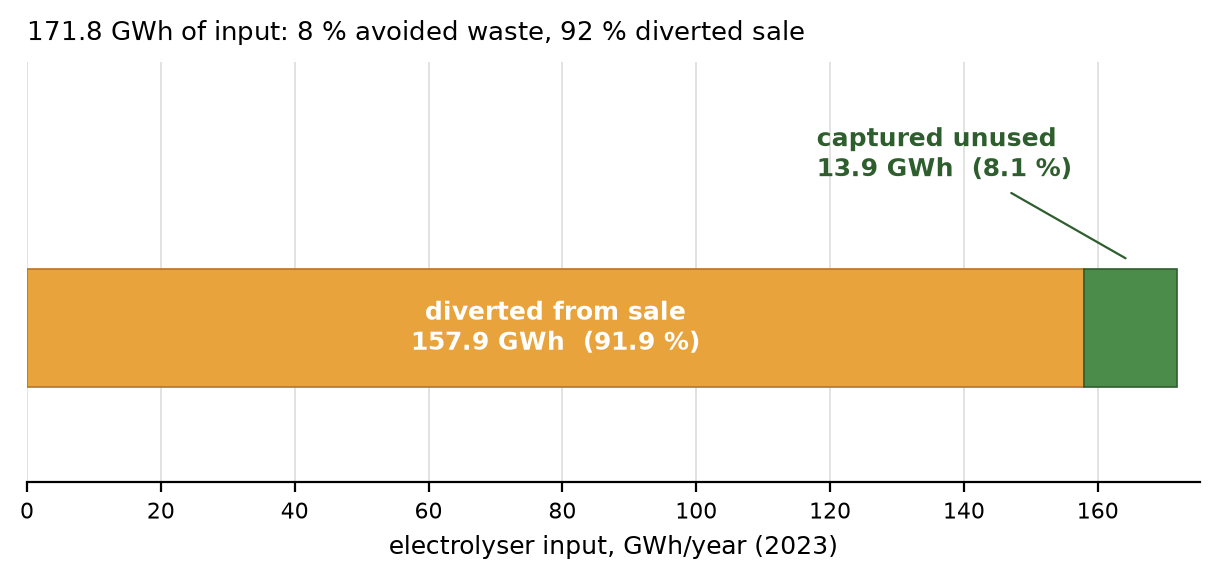
\includegraphics[width=\linewidth]{figures/fig2_attribution_redrawn.png}
\end{minipage}\hfill
\begin{minipage}[b]{0.47\linewidth}\centering
  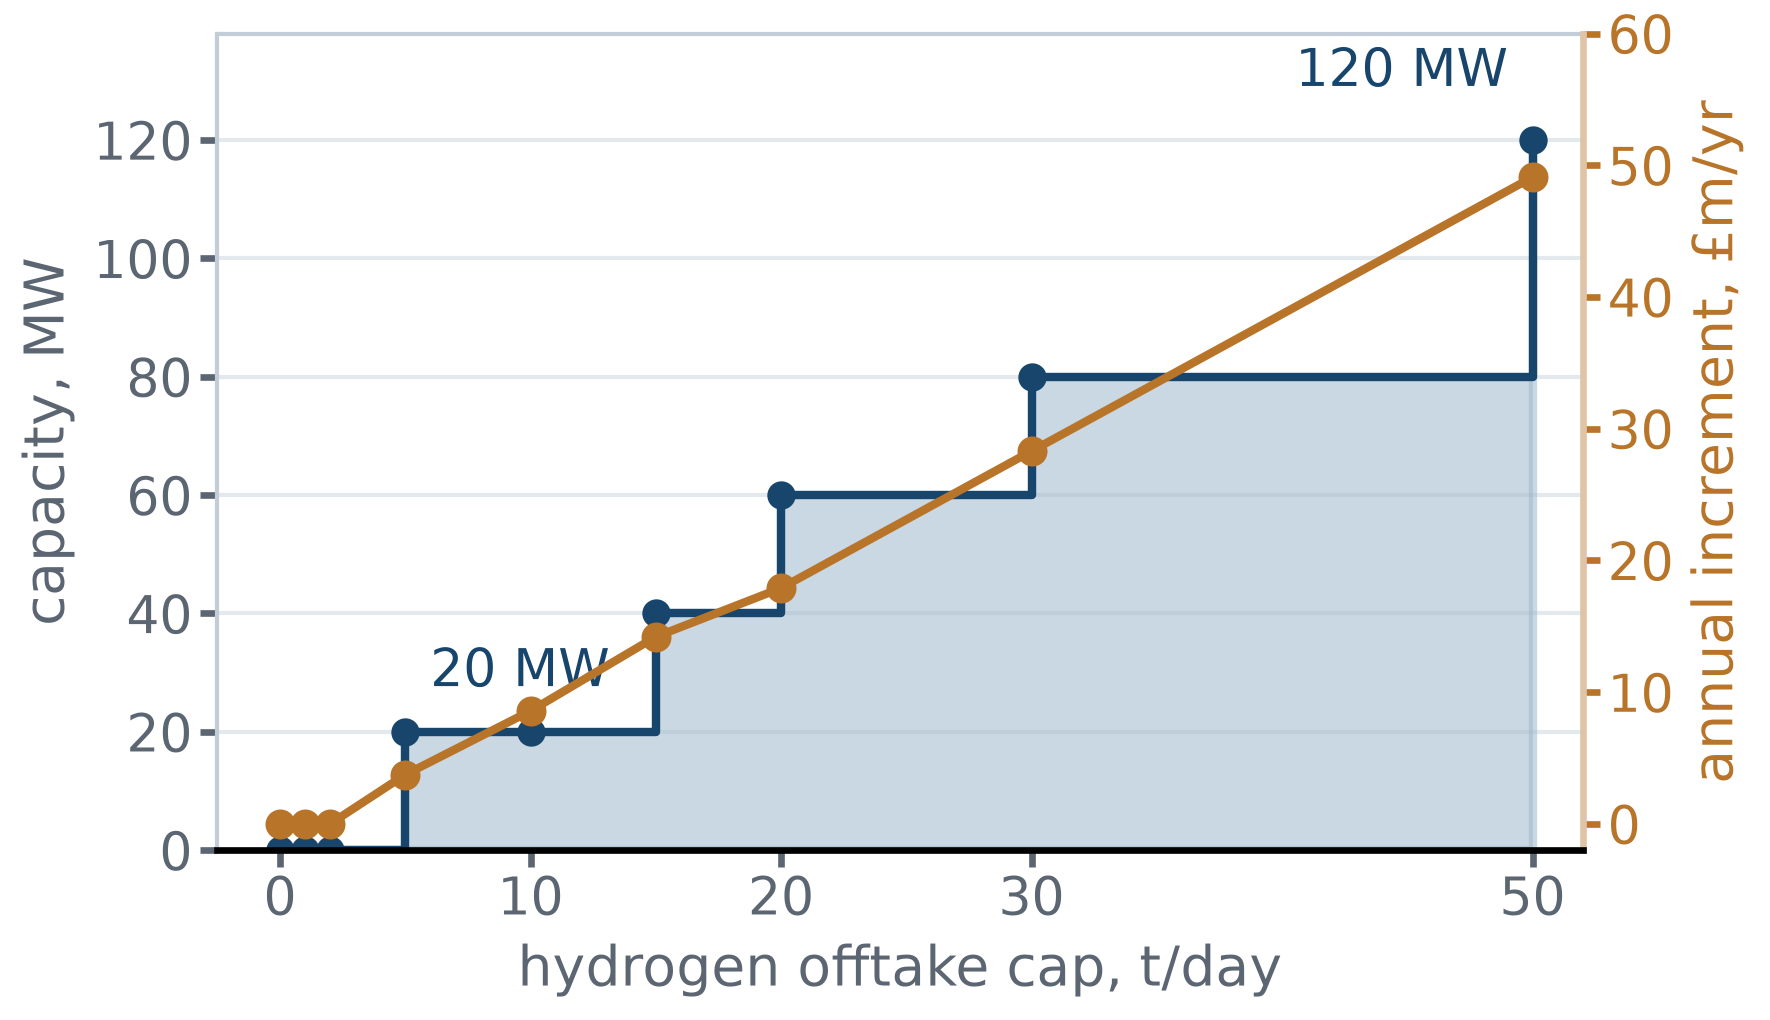
\includegraphics[width=\linewidth]{figures/fig4_ladder_redrawn.png}
\end{minipage}
\caption{Left: the 171.8\,GWh electrolyser input splits into 13.9\,GWh of otherwise-unused
generation and 157.9\,GWh diverted from sale. Right: capacity and annual increment against the
offtake cap, on a true t/day axis --- the ladder is driven by the contract, not by the surplus.
Both panels are redrawn from the package figures at printed size
(\texttt{results/results.json}); the data are unchanged.}
\label{fig:results}
\end{figure}

On the 29 surplus days the renewable share of generation is 52.7\%, so a pro-rata attribution is
about 7.3\,GWh against a strict daily bound of 0 to 13.9\,GWh. The capacity ladder follows the contract: 0\,MW at 2\,t/day or less, 20\,MW
at 5--10\,t/day, 40\,MW at 15, 60\,MW at 20, 80\,MW at 30 and 120\,MW at 50\,t/day
(+£49.1m a year on £175m of capital). At a 10\,t/day cap the investment switches on at a
netback of £4.62/kg; at £7.80/kg it needs 2{,}230\,kg/day, and at £9.5/kg (2020 money,
£11.4 at 2023 prices), 1{,}717\,kg/day. Capacity stays at 20\,MW anywhere between £7.80 and
£9.50, so the 1.4\% gap to the deflated brief benchmark does not move the decision.
Fixing 20\,MW and replaying each year keeps policy~A positive throughout, +£6.29m (2021) to
+£16.78m (2020), while policy~B loses money in 2023 and 2024 ($-$1.07m, $-$1.00m); the freedom to
allocate generation is what the asset depends on.

\needspace{7\baselineskip}
\section{What changes it, and what to do}

Electrolyser CAPEX of £0.82m--£1.65m/MW gives +£9.41m to +£8.33m with capacity unchanged; a
0--12\% real discount rate +£9.44m to +£6.99m; strict 2023 days +£8.69m; no wind farm +£8.13m;
the unrepaired price +£15.19m, which is why it is not used. None moves the decision --- the supply
obligation does.

\begin{enumerate}
  \item No battery in Tier 1 at the brief's cost. Re-open it only with intraday or ancillary
        revenue, or a capital cost near £7k/MWh.
  \item Negotiate the hydrogen contract first: at least 2.2\,t/day at £7.80/kg, or 1.7\,t/day
        at £9.5/kg. Below a £4.62/kg netback, do not build.
  \item Build 20\,MW only with the contract \emph{and} the operating mandate to divert about
        0.07\% of sales.
  \item Stage the expansion: 20\,MW for a 10\,t/day contract, 120\,MW for 50\,t/day. Do not
        pre-build, and report the capture honestly: 13.9\,GWh of avoided waste and 157.9\,GWh
        diverted from sale.
\end{enumerate}

\section{Validation and limitations}

Every stored plan (185 cases) closes its daily energy, demand, charge, discharge, module and
offtake caps, and revenues and costs are recomputed from the plans. The reference cases reproduce
the independently built Baseline 1104 package (A0 17{,}139.332; 20\,MW +8.572; fixed module
$-$1.065; 2024 +11.951) --- arithmetic agreement, not an endorsement of shared assumptions. A
third, separately written Xpress implementation of the same boundary [7] matches all 2{,}452 input
days and the 18 matched 2023--2025 cases (largest annual difference £49.54, 0.005\%) and solves the
40\,MW counterfactual at +£7.47m, below 20\,MW.

\vspace{3pt}
Limitations, measured rather than conceded: daily averages remove intraday value, so the battery
figure is an upper bound; the annual battery balance is a relaxation; dispatch is
perfect-foresight; the hydrogen value is a reference, not a contract; CAPEX is a modern midpoint
with older UK proxies for O\&M and stack renewals; no degradation, storage or ancillary market;
523 of the 2{,}452 days carry a non-strict flag, so the renewable attribution is conditional on
the repair; 2026 is partial.

\needspace{4\baselineskip}
\section*{Reproducibility and references}
{\scriptsize\raggedright\hyphenpenalty=10000\exhyphenpenalty=10000
\setlength{\columnsep}{14pt}%
\begin{multicols}{2}
\begin{enumerate}[label={[\arabic*]},leftmargin=1.8em,itemsep=1pt,topsep=2pt,parsep=0pt]
  \item Data: Group 15 data-repair release \texttt{20261104-v2}, 2,452 days, with repair log;
        accessed 4 November 2026.
  \item Brief and teacher clarifications, 2026: asset specifications and the £9.5/kg benchmark. The
        10\,t/day offtake cap is our own analysis scenario, not a term of the brief.
  \item Office for National Statistics, CPI series D7BT, monthly; all money rebased to 2020 GBP.
  \item BEIS, \emph{Hydrogen Production Costs 2021} (real 2020 GBP); IEA, \emph{Global Hydrogen
        Review 2025}; \mbox{ITM POSEIDON} data sheet: capital, fixed O\&M, stack renewal,
        55.9\,kWh/kg.
  \item Danish Energy Agency, \emph{Technology Data for Energy Storage}: installed cost, lifetime,
        O\&M and the 3\,MWh/1.5\,MW reference unit; its 0.288m EUR/MWh is the value the brief
        adopts.
  \item DESNZ, \emph{HAR1 successful projects}, December 2023: weighted strike price £241/MWh
        (£175/MWh in 2012 prices); hydrogen netback after non-power variable cost, rebased to
        2020 money.
  \item Group~15's independently written Xpress implementation B, Tier~1 workspace, commit
        \texttt{71ce76e}; the cross-implementation result is reported in Section~6.
\end{enumerate}
\end{multicols}}

\end{document}
